\documentclass{article}
\usepackage[paperwidth=8in,paperheight=10in, margin=0.5in]{geometry}


\usepackage[utf8]{inputenc}
\usepackage[T1]{fontenc}
\usepackage{graphicx}
\usepackage{makeidx}

\makeindex

\usepackage[english]{babel}

\title{SPACE ATTACK}
\author{Marcus Karpoff}
\date{}

\begin{document}

\maketitle

\pagebreak

\tableofcontents

\pagebreak

\section{Story}

\subsection{Introduction}
In the year 2028 humanity found out that they weren't alone. They came when we 
least expected it. Most of the world is dead from the alien landing parties. We
have discovered that there is one advantage we have on them. The have no bombs.
We have one last line of defence. You! God help us.

\subsection{Who are you?}
You are the gunner controlling the last city's last turret. Your job is simple... Defend the city... or suffer the children.

\subsection{Who are they?}
Nobody knows all we know is that every city they get to ends up empty. We must 
keep them out... think of the children...

\section{Controls}
Depending on whether or not the version of Unix, they type of command line 
interface you use, and what version of ncurses is available will determine 
whether or not you will be able to default interface.

\subsection*{If your version of Unix and curses supports special key presses:}
LEFT ARROW - Will cause your turret to move to the left.\\
RIGHT ARROW - Will cause your turret to move to the left.\\
DOWN ARROW - Will cause your turret to jump to the very end.\\
UP ARROW - Will cause your turret to jump to the very beginning.\\
SPACE - Fire the rocket!\\
Q - Quit and let the children suffer.

\subsection*{If your version of Unix or curses doesn't support special key 
presses:}
, - Will cause your turret to move to the left.\\
. - Will cause your turret to move to the left.\\
/ - Will cause your turret to jump to the very end.\\
m - Will cause your turret to jump to the very beginning.\\
SPACE - Fire the rocket!\\
Q - Quit and let the children suffer.

\pagebreak
\section{Interface}

 \centerline{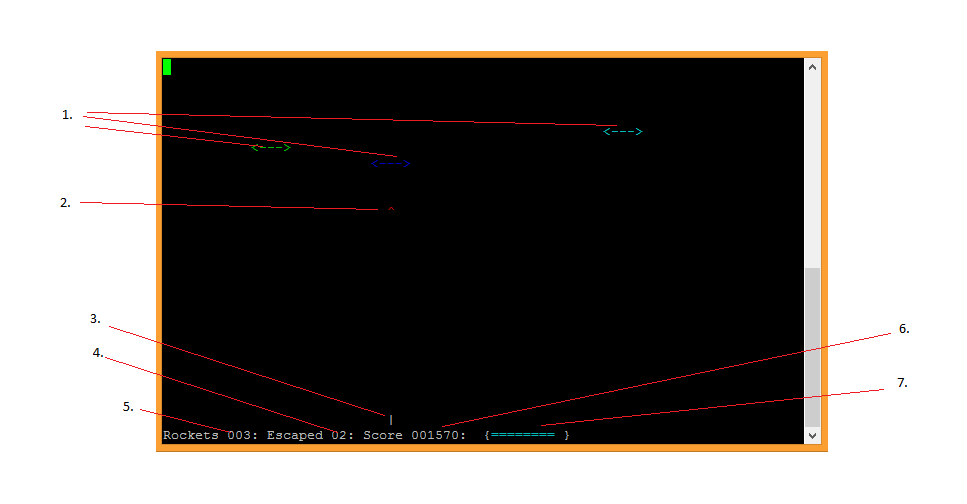
\includegraphics[width=\paperwidth]{saucerUI.png}}
1........Saucers\\
2........Rockets\\
3........Turret\\
4........Escaped Counter\\
5........Rocket Counter\\
6........Score Board\\
7........Bonus Rocket Gauge \\
\subsection{Saucers}
The saucers are the enemy's ships. You fire rockets at these ships to blow them
up. The different ships colours represent how fast they are categorically. If 
10 of these ships gets to the right edge of the screen then there are enough 
alien troops landed to overrun the infantry. If this happens then you have 
failed the last citizens and they will raze the city... think of the children...

\subsection{Rockets}
These suckers pack enough of a punch to blow up a alien ship with a single hit.
Unfortunately we are running low of them. For every enemy ship you hit you will
get only 1 extra rocket so don't miss or all is lost... think of the children...

\subsection{Turret}
This is your turret. You can move it left and right using the appropriate 
keys. When a rocket is launched it is always launched from the location that 
the turret was at at launch time. So position the turret carefully or you will
was rockets... and our hopes...

\subsection{Escaped}
This counter counts the number of rockets that have gotten past you. If this gets to 10 all the citizens are going to die.

\subsection{Rockets}
This counter shows how many rockets you have left. You start with 10 rockets. 
If you run out of rockets then the there is nothing stopping the aliens, so 
don't waste any because you don't have many.

\subsection{Score}
This counter shows your score. You get points for every ship you destroy. The 
faster the ship the more points you get.

\subsection{Bonus Bar}
This bar fills up slowly. When it is full you get a bonus rocket. The one thing 
that will help you, so DON'T WASTE IT.

\pagebreak

\section{Requirements}
This game will only run Unix systems that support posix threads.\\
This game requires ncurses (libncurses5-dev to build)\\
This game also requires a terminal window that is 80 x 21 in size.\\




\end{document}
